\section{سروو موتور}
\subsection{اهداف آزمایش}
\begin{itemize}
    \item آشنایی با سروو موتور
    \item آشنایی با \lr{PWM}
    \item آشنایی با مقاومت های حساس به نور
\end{itemize}
\subsection{قطعات مورد نیاز}
\begin{itemize}
    \item \lr{Arduino Uno}
    \item سروو موتور
    \item مقاومت حساس به نور (فوتوسل)
    \item مقاومت ۱۰ کیلواهم
\end{itemize}

\subsection{مقدمه}
\begin{nas}سروو موتور \end{nas}
\paragraph{سروو موتور ها یک نوع از موتور های الکتریکی هستند که به جای چرخیدن، خود را در یک زاویه خاص نگه می‌دارند. این نوع موتور ها در رباتیک کاربرد بسیار زیادی دارند. برای مثال در ساخت دست مصنوعی، ربات های مونتاژ و هر جایی که نیاز داریم چیزی را در یک زاویه خاص قرار دهیم می‌توانیم از سروو موتور استفاده کنید.
}
\paragraph{
سروو موتور ها ۳ ورودی دارند، یکی برای \lr{VCC} که معمولا یک سیم قرمز رنگ است، یکی برای \lr{GND} که معمولا قهوه‌ای یا سیاه رنگ است و سیم سوم که ورودی کنترلی را می‌گیرد. ورودی کنترلی سروو موتور به صورت یک سیگنال \lr{PWM} است و با هر چه \lr{Duty Cycle} بیشتر باشد سروو موتور در زاویه بیشتری قرار می‌گیرد.
}

\paragraph{
\textcolor{red}{\begin{nas}سوال: \end{nas}}
دیتاشیت سروو موتور \lr{SG90} را مطالعه کنید و به سوالات زیر پاسخ دهید:
}
\begin{itemize}
    \item دوره تناوب سیگنال \lr{PWM} چند است؟
    \item دامنه حرکتی این موتور ۱۸۰ درجه است. برای حالاتی که سروو موتور وسط، سمت چپ و یا سمت راست است \lr{Duty Cycle} را محاسبه کنید.
\end{itemize}


\paragraph{
\textcolor{red}{\begin{nas}سوال: \end{nas}}
برای کار با سروو موتور از کتاب‌خانه‌ی \lr{Servo.h} استفاده می‌کنیم. در مستندات این کتاب‌خانه تحقیق کنید و در مورد ورودی، خروجی و کارکرد توابع زیر توضیح دهید.
}
\begin{itemize}
    \item \lr{attach()}
    \item \lr{write()}
\end{itemize}

\begin{nas}مقاومت حساس به نور\end{nas}
\newline
مقاومت های حساس به نور یا فوتورزیستور یا فوتوسل نوعی از مقاومت متغیر است که مقدار مقاومت آن نسبت به نوری که به آن تابیده می‌شود تغییر می‌کند. مقاومت یک فوتوسل در تاریکی زیاد و در روشنایی کم می‌شود. برای اتصال آن به آردوینو می‌توانیم از یک مقاومت \lr{Pull Down} استفاده کنیم.
\newline
\textcolor{red}{\begin{nas}سوال: \end{nas}}
مدار زیر را در نظر بگیرید. اگر مقاومت فوتوسل ۱۰۰ اهم باشد ولتاژ خروجی چند است؟ اگر ۱۰۰ کیلواهم باشد چه؟
\newline
\begin{figure}[h]
    \centering
    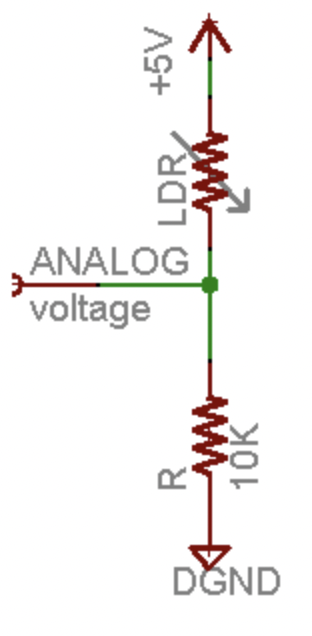
\includegraphics[width=4cm]{ldr-circ.png}
    \caption{مدار اتصال فوتوسل به آردوینو}
    \label{fig:ldr-circ}
\end{figure}
\pagebreak

\subsection{شرح آزمایش}
\begin{enumerate}
    \item فوتوسل را مانند مداری که در مقدمه بررسی کردید به آردوینو متصل کنید. مشخصا باید \lr{Analog Voltage} را به یکی از پین های ورودی آنالوگ متصل کنید.
    \item برنامه‌ای بنویسید که با آن بفهمید خروجی \lr{analogRead} هنگامی که بر روی فوتوسل نور می‌تابد و هنگامی که دستتان را روی آن گرفتید چند است.
    \item سروو را به آردوینو وصل کنید. سیم های \lr{VCC} و \lr{GND} را به ولتاژ ۵ ولت و زمین وصل کنید و سیم کنترلی را به یکی از پین های \lr{PWM} آردوینو. برای این کار می‌توانید از پین های ۹ یا ۱۰ استفاده کنید.
    \item برنامه‌ای بنویسید که ولتاژ فوتوسل را بخواند، اگر مقدار آن ۱۰ درصد کمتر از ولتاژ حالت تاریک باشد زاویه سروو موتور را صفر درجه و اگر مقدار آن ۱۰ درصد بیشتر از ولتاژ حالت روشن باشد زاویه سروو موتور را ۱۸۰ درجه کند. برای این کار می‌توانید از تابع \lr{map} استفاده کنید.
\end{enumerate}